\chapter{Background \& Objectives}

This section should discuss your preparation for the project, including background reading, your analysis of the problem and the process or method you have followed to help structure your work.  It is likely that you will reuse part of your outline project specification, but at this point in the project you should have more to talk about. 

\textbf{Note}: 

\begin{itemize}
   \item All of the sections and text in this example are for illustration purposes. The main Chapters are a good starting point, but the content and actual sections that you include are likely to be different.
   
   \item Look at the document on the Structure of the Final Report for additional guidance. 
   
\end {itemize}

\section{Background}
What was your background preparation for the project? What similar systems did you assess? What was your motivation and interest in this project? 

%we looked mostly at zegami and the access-phenomics site, these were the similar systems that we researched primarily

\section{Analysis}
Taking into account the problem and what you learned from the background work, what was your analysis of the problem? How did your analysis help to decompose the problem into the main tasks that you would undertake? Were there alternative approaches? Why did you choose one approach compared to the alternatives? 

There should be a clear statement of the objectives of the work, which you will evaluate at the end of the work. 

In most cases, the agreed objectives or requirements will be the result of a compromise between what would ideally have been produced and what was felt to be possible in the time available. A discussion of the process of arriving at the final list is usually appropriate.

\section{Process}
%You need to describe briefly the life cycle model or research method that you used. You do not need to write about all of the different process models that you are aware of. Focus on the process model that you have used. It is possible that you needed to adapt an existing process model to suit your project; clearly identify what you used and how you adapted it for your needs.

Plan driven approaches traditionally associated with software development projects usually expect that all system requirements are understood and collected prior to any further work on design or implementation. A number of factors made such an approach unsuitable for this project, chiefly a lack of domain knowledge made up-front requirement gathering difficult and the requirements themselves were likely to be poorly defined and subject to change. With these considerations in mind it was decided that an agile approach would be best. 

A SCRUM-inspired approach was adopted for the project methodology, featuring time-boxed iterations in the form of sprints with regular releases of the software. Work would be tracked in the form of user-stories, the planning and organisation of work would revolve around a defined functionality goal for each sprint and release.  

\begin{figure}[H]
    \centering
    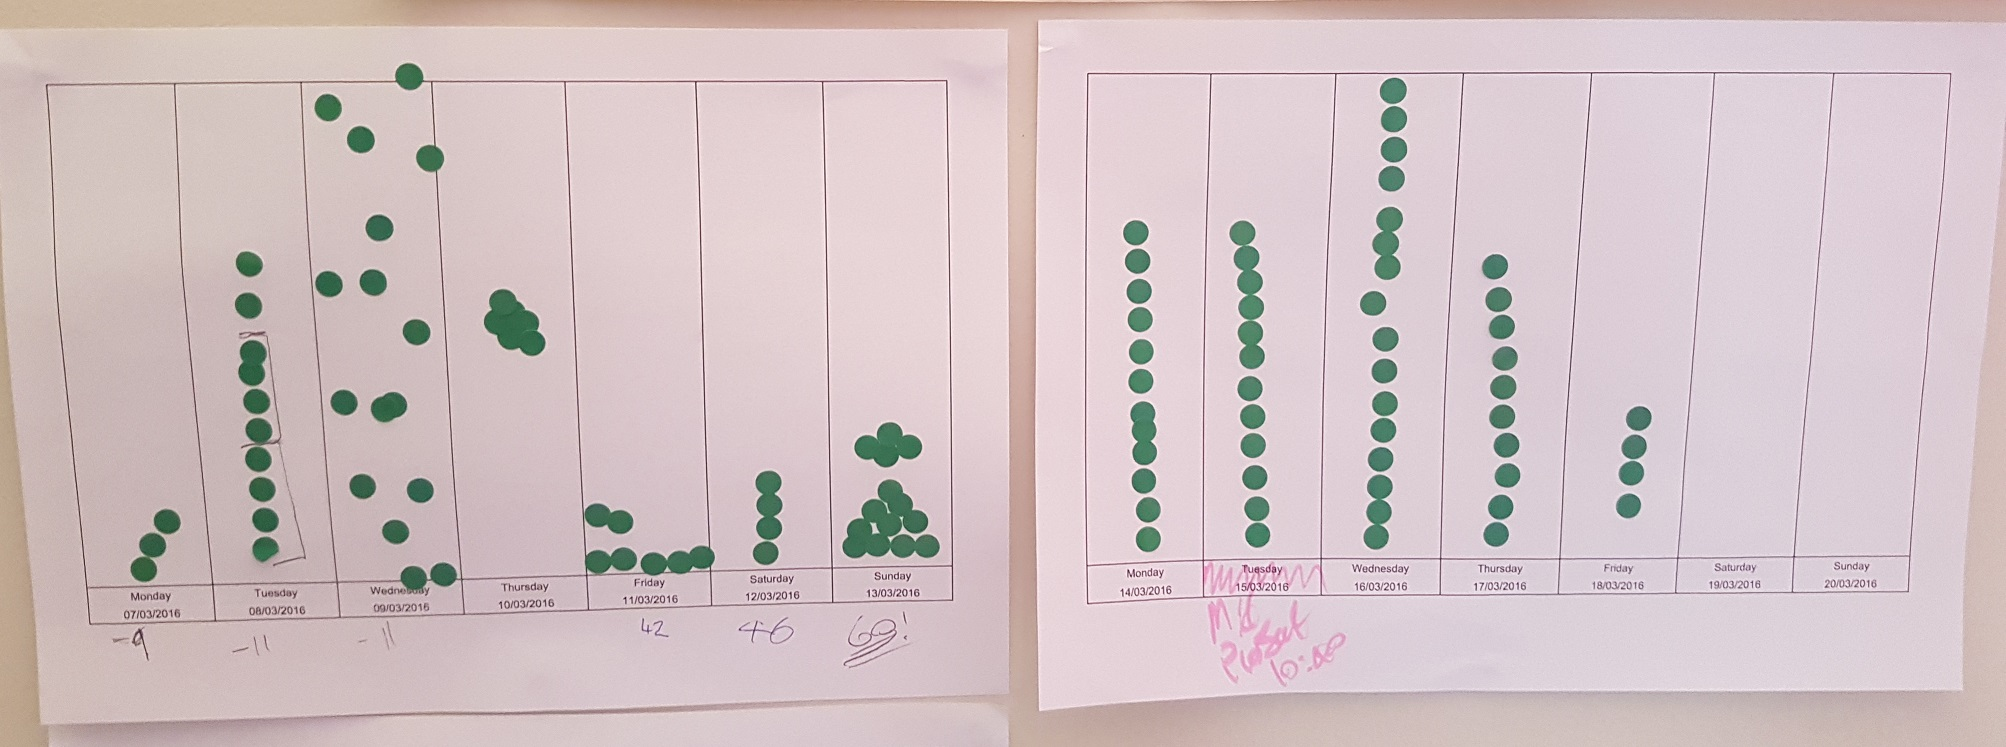
\includegraphics[width=\textwidth]{images/process/pomotrack}
    \caption{Tracking pomodoros}
    \label{fig:pomo1}
\end{figure}


%The process used for the project was an agile based approach similar in style to Scrum although adapted for a project team of one. The process centred around User Stories and short iterations of one week. 

